\documentclass[11pt,a4paper]{article}
\usepackage[margin=2.4cm]{geometry}
\usepackage{amsmath,amssymb,amsthm,bm}
\usepackage{graphicx}
\usepackage{booktabs}
\usepackage{xcolor}
\usepackage{listings}
\usepackage[colorlinks=true,linkcolor=blue!60!black,citecolor=blue!60!black,urlcolor=blue!60!black]{hyperref}
\usepackage{caption}
\captionsetup{font=small,labelfont=bf}
\graphicspath{{figures/}}

\newtheorem{proposition}{Proposition}
\newtheorem{definition}{Definition}
\theoremstyle{remark}
\newtheorem{remark}{Remark}

\newcommand{\uu}{\bm{u}}
\newcommand{\ub}{\uu_b}
\newcommand{\nn}{\bm{n}}
\newcommand{\Sf}{\bm{S}_f}
\newcommand{\Sw}{\bm{S}_w}
\newcommand{\dd}{\,\mathrm{d}}
\newcommand{\dt}{\Delta t}
\newcommand{\Aw}{A_{\rm wall}}
\newcommand{\dw}{d_{\rm wall}}
\newcommand{\code}[1]{\texttt{#1}}

\lstset{basicstyle=\footnotesize\ttfamily,columns=fullflexible,keepspaces=true,frame=single,framerule=0.3pt,xleftmargin=1em}

\title{\bf A cut-cell immersed boundary method for static and moving bodies\\
in a collocated finite-volume solver\\[3pt]
\large Formulation, implementation in OpenFOAM and verification}
\author{}
\date{\today}

\begin{document}
\maketitle

\begin{abstract}
We present a cut-cell immersed boundary method for the incompressible Navier--Stokes
equations on a fixed, non body-fitted mesh, its extension to rigid bodies moving through the
mesh, and the transport of a passive scalar in the same framework. The body is described by
a level set; each face of the mesh carries the fraction of its area that lies in the fluid
and each cell the fraction of its volume. The wall segment of a cut cell is not computed
independently but \emph{defined} by the geometric closure of the fluid polyhedron, and this
single identity carries the whole boundary treatment: the wall pressure force is absorbed
into a face sum, no-penetration follows from discrete continuity, and the difference between
a free-slip and a no-slip wall is one diagonal coefficient. No ghost values, no extrapolation
into the solid and no coupling between velocity components appear. For a moving body only
continuity changes: it acquires the flux swept by the wall as a source, and taking that flux
--- rather than the geometric volume change --- as the primary quantity makes the discrete
geometric conservation law hold by construction, so that a free stream is preserved to machine
precision at any body speed. A passive scalar is transported by the same face fluxes and sees
the wall either as a fixed-value or as a zero-flux surface, and its budget closes to round-off.
The method is implemented in OpenFOAM without modifying the mesh: the fractions enter the
standard operators explicitly, which keeps the pressure--velocity coupling of
\code{simpleFoam}/\code{pimpleFoam} and the linear algebra untouched, and the whole
moving-body extension sits behind a single run-time switch. The implementation is verified
against an independent reference implementation of the same discretisation on a cylinder at
$Re_D=1$ at rest, oscillating and translating through a periodic seam, and by conservation
tests for the scalar.
\end{abstract}

\tableofcontents

\section{Introduction}

Immersed boundary methods let a body of arbitrary shape be represented on a mesh that does
not conform to it. Among them, cut-cell methods are distinguished by being conservative:
the fluid part of every cell is a well-defined control volume, and fluxes are accounted for on
its actual boundary. Their classical difficulties are the description of the cut geometry, the
small-cell problem, and, for moving bodies, the consistency between the change of the fluid
volume of a cell and the flux swept by its wall, i.e.\ the discrete geometric conservation law.

The method described here addresses these points with a minimum of machinery. Its central
object is the \emph{closure identity} of a cut cell: the wet parts of its faces and its wall
segment form a closed surface, so the wall area vector equals minus the sum of the wet face
area vectors. Rather than computing the wall segment from the geometry and then enforcing
consistency, the method defines the wall segment through the identity. Every consequence of
the boundary condition --- pressure force, no-penetration, wall traction, and for a moving body
the volume swept --- is then expressed with the same face fractions that the flux operators
use, and the resulting discrete properties (exactness for uniform flow, no spurious force from
a uniform pressure, exact compatibility of the pressure system, free-stream preservation) hold
to round-off by construction.

Section~\ref{sec:geom} defines the geometry and its computation, Section~\ref{sec:static}
the discretisation for a body at rest, Section~\ref{sec:moving} the extension to moving
bodies, Section~\ref{sec:scalar} the transport of a passive scalar. Section~\ref{sec:impl}
describes the implementation in OpenFOAM, Section~\ref{sec:verif} the verification, and
Section~\ref{sec:limits} the limitations.

\section{Governing equations}

We solve the incompressible Navier--Stokes equations
\begin{equation}
\frac{\partial \uu}{\partial t}+\nabla\!\cdot\!(\uu\uu)-\nabla\!\cdot\!(\nu\nabla\uu)
=-\nabla p+\bm{g},
\qquad \nabla\!\cdot\!\uu=0,
\label{eq:ns}
\end{equation}
with $p$ the kinematic pressure and $\bm{g}$ a body force, in a domain $\Omega$ containing
one or more rigid bodies $B_i$ with prescribed velocity $\ub(\bm x,t)$ (zero for a body at
rest, $\bm U(t)+\bm\omega\times(\bm x-\bm c(t))$ for a rigid body). On each body surface one
of two conditions is imposed: \emph{no slip}, $\uu=\ub$, or \emph{free slip},
$(\uu-\ub)\cdot\nn=0$ together with zero tangential traction. A passive scalar $T$ obeys
\begin{equation}
\frac{\partial T}{\partial t}+\nabla\!\cdot\!(\uu T)-\nabla\!\cdot\!(D\nabla T)=q,
\label{eq:scalar}
\end{equation}
with, on the body, either a fixed value $T=T_w$ or zero diffusive flux
$\partial T/\partial n=0$.

The discretisation is a collocated finite-volume method with SIMPLE(C) pressure--velocity
coupling in the arrangement of OpenFOAM's \code{simpleFoam} (steady) and \code{pimpleFoam}
(transient, implicit Euler with outer iterations). We write $V_P$ for the volume of cell $P$,
$\Sf$ for the area vector of face $f$ pointing out of $P$, $\phi_f$ for the volume flux
through $f$, and $\delta_f=1/|\bm d_f|$ for the inverse of the centre-to-centre distance across
$f$. Face values are linear interpolates, $(\cdot)_f=\tfrac12[(\cdot)_P+(\cdot)_N]$ on a
uniform mesh.

\section{Geometric description of the body}
\label{sec:geom}

\subsection{Fluid fractions and the closure identity}

\begin{definition}[Level set and fractions]
A body is given by a function $\varphi(\bm x)$, negative inside the body and positive in the
fluid; only its sign and its zero level are used. For a face $f$ and a cell $P$,
\begin{equation}
\theta_f=\frac{|\{\bm x\in f:\varphi>0\}|}{|f|}\in[0,1],\qquad
\alpha_P=\frac{|\{\bm x\in P:\varphi>0\}|}{V_P}\in[0,1]
\end{equation}
are the fluid area and volume fractions. A cell is fluid if $\alpha_P=1$, solid if
$\alpha_P=0$, cut otherwise. Several bodies are combined through the minimum of their level
sets, which represents their union exactly.
\end{definition}

The fluid part $\Omega_P$ of a cut cell is a polyhedron bounded by the wet parts of the cell
faces, of area vectors $\theta_f\Sf$, and by the wall segment, of area $\Aw$ and outward unit
normal $\nn_w$ (Fig.~\ref{fig:cutcell}).

\begin{figure}[htbp]\centering
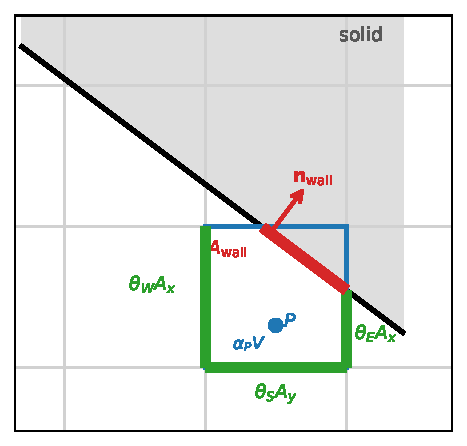
\includegraphics[width=0.55\textwidth]{f1_cutcell.pdf}
\caption{A cut cell. The fluid boundary consists of the wet parts of the faces (areas
$\theta_f|\Sf|$) and the wall segment (area $\Aw$, outward normal $\nn_w$). The cell carries
fluid volume $\alpha_PV_P$.}
\label{fig:cutcell}
\end{figure}

\begin{proposition}[Closure]
\label{prop:closure}
For every cut cell, $\sum_f\theta_f\Sf+\nn_w\Aw=\bm 0$.
\end{proposition}
\begin{proof}
Apply the divergence theorem to a constant vector field over $\Omega_P$.
\end{proof}

We write $\Sw\equiv-\sum_f\theta_f\Sf=\nn_w\Aw$ for the wall area vector, pointing from the
fluid into the body, and $\Aw=|\Sw|$. In the implementation $\Sw$ is never computed from the
level set: it is \emph{defined} by Proposition~\ref{prop:closure} from the same $\theta_f$ that
weight every flux operator, so the identity holds to round-off, however the wall is inclined
and, for a moving body, however fast it moves.

Two further derived quantities are needed. The effective wall-normal distance of the cell
average from the wall is estimated from the volume the cell holds behind its wall segment,
halved for a profile linear in the wall-normal direction,
\begin{equation}
\dw=\frac{\alpha_PV_P}{2\Aw},
\label{eq:dwall}
\end{equation}
and the \emph{Dirichlet wall coefficient} $\Aw/(\dw V_P)=2\Aw^2/(\alpha_PV_P^2)$, which
multiplies a diffusivity to give the wall exchange coefficient per unit volume.
A fluid cell one of whose faces is fully closed by a solid neighbour has $\Sw\neq\bm 0$ as
well; it is treated as a wall cell with $\dw=h/2$, the staircase limit of the same formula.

\subsection{Computation}
\label{sec:geomcomp}

The fractions are computed once for a body at rest and at every time step for a moving body,
as follows.
\begin{enumerate}\itemsep2pt
\item The level set is evaluated at the mesh points, the face centres and the cell centres.
\item On every edge whose end points differ in sign, the crossing is located by bisection of
      the exact level set (40 steps, i.e.\ to machine precision relative to the edge length).
      The bisection runs in a canonical direction along the edge so that the two sides of a
      processor or periodic boundary obtain the same crossing.
\item $\theta_f$ is the area of the fluid polygon of the face (fluid vertices and crossing
      points, in order) divided by $|\Sf|$.
\item $\alpha_P$ is obtained by sub-sampling the level set on a lattice of $n_s^d$ points in
      the cell ($n_s=32$ here; $d$ is the number of solution directions, so a two-dimensional
      case samples a $32\times32$ lattice), for every cell whose vertices, face centres and
      centre do not all lie on the same side. A body smaller than a cell is not resolved.
\item \emph{Sliver absorption.} Cells with $\alpha_P<\alpha_{\min}$ (here $0.02$) are
      absorbed into the body: $\alpha_P:=0$ and \emph{all their faces are closed},
      $\theta_f:=0$. Closing the faces is essential: an absorbed cell with an open face would
      break Proposition~\ref{prop:closure} for its neighbours, which would then see a flux
      into a cell that carries no equation. The absorption displaces the boundary by
      $O(\alpha_{\min}h)$, within the first-order error of the no-slip treatment.
\item \emph{Coupled faces.} The two copies of a face on a periodic or processor boundary must
      carry the same fraction. After absorption, $\theta_f$ is synchronised across coupled
      faces with the minimum, which also propagates the closing of absorbed cells across the
      boundary. Doing this \emph{after} absorption matters (Section~\ref{sec:galilean}).
\end{enumerate}
Bodies described by a closed triangulated surface use the signed distance to the surface as
level set (nearest point and inside/outside test), so that the same bisection applies. A body
given only as a fluid-fraction field $\alpha$ has its face fractions reconstructed from the
$0.5$ iso-surface of the point-interpolated field; this route is less accurate
(Section~\ref{sec:limits}) and is intended for fractions produced by another model.

\subsection{Multiple bodies}

The level sets of all bodies are combined by their minimum before the fractions are computed,
so overlapping bodies form an exact union. Every cut, solid or wall cell is attributed to a
body --- the one with the smallest level set at its centre, or the one across its closed face
--- which selects the wall condition (no slip or free slip; fixed value or zero flux for the
scalar), the wall velocity, and the body to which its force contribution is added.

\section{Discretisation for a body at rest}
\label{sec:static}

Every term of \eqref{eq:ns} is integrated over the fluid part $\Omega_P$ of each cell. The
wall segment contributes to each term according to the boundary condition, and this is the
only place where the boundary condition enters. Table~\ref{tab:static} collects the result.

\begin{table}[htbp]\centering\small
\caption{Volume-integrated terms on the fluid part of a cell; $\Gamma$ is a diffusivity,
$p_f$ and $\bar\uu_f$ are linear face interpolates.}
\label{tab:static}
\begin{tabular}{@{}lll@{}}
\toprule
term & wall contribution & discrete operator\\
\midrule
unsteady & --- & $\alpha_PV_P\,(\uu_P^{n+1}-\uu_P^{n})/\dt$\\[3pt]
convective & zero ($\uu\cdot\nn_w=0$) & $\sum_f\phi_f\,\bar\uu_f$, \quad $\phi_f=\theta_f\,\bar\uu_f\cdot\Sf$\\[3pt]
viscous, free slip & zero (no tangential traction) & $\sum_f\theta_f\,\Gamma_f\,\delta_f|\Sf|\,(\uu_N-\uu_P)$\\[3pt]
viscous, no slip & $\nu\,(\bm 0-\uu_P)\Aw/\dw$ & same, plus $-\nu\,\Aw/\dw\,\uu_P$\\[3pt]
pressure & $p_P\Sw$, absorbed by closure & $\sum_f\theta_f\,(p_f-p_P)\,\Sf$\\[3pt]
continuity & zero & $\sum_f\phi_f=0$\\
\bottomrule
\end{tabular}
\end{table}

The pressure entry deserves a derivation. The volume-integrated gradient is
$\oint_{\partial\Omega_P}p\,\nn\dd S$; splitting the boundary into the wet faces and the wall
segment, and taking $p_w=p_P$ on the wall to first order,
\begin{equation}
\oint p\,\nn\dd S=\sum_f\theta_fp_f\Sf+p_P\Sw
\overset{\text{Prop.\,\ref{prop:closure}}}{=}\sum_f\theta_f\,(p_f-p_P)\,\Sf .
\label{eq:grad}
\end{equation}
The wall pressure force --- the form drag --- is therefore absorbed exactly into the face sum,
and a uniform pressure produces no force on any cell.

\subsection{Properties}

\begin{proposition}[Exactness for uniform tangential flow]
For a plane wall and a uniform discrete velocity $\uu$ with $\uu\cdot\nn_w=0$, the discrete
divergence vanishes identically in every cut cell.
\end{proposition}
\begin{proof}
$\sum_f\phi_f=\uu\cdot\sum_f\theta_f\Sf=-\uu\cdot\Sw=0$.
\end{proof}

\begin{proposition}[No-penetration is implied, not imposed]
\label{prop:nopen}
For a locally uniform $\uu$ in a cut cell with $\Aw\neq0$, discrete continuity
$\sum_f\phi_f=0$ holds if and only if $\uu\cdot\nn_w=0$.
\end{proposition}

Proposition~\ref{prop:nopen} is the structural point of the method: the no-penetration
condition is never written down, it is a consequence of enforcing mass conservation on the cut
cell with fluxes and wall segment taken from the same fractions. The free-slip condition
appears only as the \emph{absence} of a wall term in the viscous operator, and the no-slip
condition as the presence of the single diagonal term $\nu\Aw/\dw$. Because
$\dw\propto\alpha_P$, this coefficient grows like $1/\alpha_P$ as a cell is squeezed against
the wall: the small-cell limit \emph{strengthens} diagonal dominance and drives $\uu_P$ onto
the wall value rather than degrading the system. Consequently the discretisation contains no
ghost value, no extrapolation into the solid, no blanking of cut cells, no coupling between the
velocity components, and no adjustable parameter other than $\alpha_{\min}$.

Measured against exact solutions of Poisson problems on a disk, the free-slip treatment is
second-order accurate and the no-slip treatment first-order accurate, the difference being
entirely due to the wall-normal distance estimate \eqref{eq:dwall}, which free slip does not
need.

\subsection{Solid cells and the pressure--velocity coupling}
\label{sec:coupling}

Every face of a solid cell is closed, so its rows in the momentum and pressure matrices are
empty. The momentum row receives a blanking diagonal $\nu\sum_f|\Sf|\delta_f/V_P$ (the
viscous diagonal of an unobstructed cell) and the source that drives the cell to the body
velocity; the pressure row receives a diagonal of the typical magnitude of the fluid rows and a
zero source, so that $p=0$ there. Neither value affects the fluid: the rows are decoupled.

The coupling is SIMPLEC. Writing the assembled momentum equation of cell $P$ as
$a_P\uu_P=\bm H(\uu)-\nabla_{\!V}p$, with $\nabla_{\!V}p$ the volume-integrated gradient
\eqref{eq:grad} and $\bm H=\bm b-\sum_{nb}a_{nb}\uu_{nb}$,
\begin{equation}
r_{A}=\frac{V_P}{a_P},\qquad
r_{At}=\frac{V_P}{a_P+\sum_{nb}a_{nb}},\qquad
\sum_f\theta_f\,(r_{At})_f\,\delta_f|\Sf|\,(p_N-p_P)=\sum_f\phi_{H,f}+S_P,
\label{eq:peqn}
\end{equation}
where $\phi_{H,f}=\theta_f\,(\bm H/a_P)_f\cdot\Sf+\theta_f\,(r_{At}-r_A)_f\,\delta_f|\Sf|(p^{\rm old}_N-p^{\rm old}_P)$
is the Rhie--Chow flux of the predictor, and $S_P$ is the mass source of a moving wall
(zero for a body at rest, Section~\ref{sec:moving}). The corrected flux
$\phi_f=\phi_{H,f}-\theta_f(r_{At})_f\delta_f|\Sf|(p_N-p_P)$ is then discretely
divergence-free, and the velocity is corrected with the gradient \eqref{eq:grad}. Laplacian
and flux in \eqref{eq:peqn} are weighted by the same $\theta_f$, so no inconsistency
appears at the wall. The denominator of $r_{At}$ is floored at the transient diagonal
$\alpha_PV_P/\dt$ (the value of an unobstructed cell) to keep the pressure Laplacian definite.

The fluid region is a pure Neumann island for the pressure, and the reference is imposed as
in \code{fvMatrix::setReference}, by doubling one diagonal entry rather than replacing a row.
With $L$ the pressure matrix on the fluid cells ($\bm 1^{\!\top}L=\bm 0$) and
$L'=L+d_r\bm e_r\bm e_r^{\!\top}$, left-multiplying $L'p=\bm b$ by $\bm 1^{\!\top}$ gives
$d_rp_r=\bm 1^{\!\top}\bm b$: for a compatible right-hand side the reference is transparent
and $Lp=\bm b$ exactly, whereas any incompatibility is deposited at the reference cell as a
spurious point source. Exact compatibility of $S_P$ is therefore not a nicety but a
requirement (Section~\ref{sec:primary}).

\subsection{Force on the body}

By closure, the pressure force on a body is $\bm F_p=\sum_Pp_P\Sw$ over its wall cells, and
the viscous force is the reaction to the traction already assembled in the momentum equation,
$\bm F_v=\sum_P\nu\,\Aw/\dw\,(\uu_P-\ub)$ for no slip and zero for free slip. Summing the
momentum equations over the fluid shows that, at steady state in a periodic domain, the total
force equals the driving body force times the fluid volume exactly; this identity is used as a
consistency check in Section~\ref{sec:verif}.

\section{Moving bodies}
\label{sec:moving}

\subsection{What the wall sweeps}

The mesh never moves: no face carries a mesh velocity and no mesh-motion term appears in any
operator, so the method is not an arbitrary Lagrangian--Eulerian scheme. Only $\theta_f$,
$\alpha_P$ and $\Sw$ depend on time, and they are recomputed from the level set at every time
step. The entire modification lives on the wall segment.

Let $\Omega_P(t)$ be the fluid part of cell $P$. Its boundary consists of the wet parts of the
faces, which lie in fixed planes and sweep no volume, and the wall segment, which moves with
$\ub$. Reynolds transport gives
\begin{equation}
\frac{\dd(\alpha_PV_P)}{\dd t}=\int_{\rm wall}\ub\cdot\nn_w\dd S\simeq\ub\cdot\Sw ,
\label{eq:volume}
\end{equation}
and continuity over the same region, with $(\uu-\ub)\cdot\nn_w=0$ on the wall,
\begin{equation}
\boxed{\;\sum_f\theta_f\phi_f=-\,\ub\cdot\Sw\equiv-S_P .\;}
\label{eq:continuity}
\end{equation}
The sign is as it must be: a body advancing into the fluid has $\ub\cdot\nn_w<0$, the cell
loses volume, and the net outflow through its faces is positive.

\begin{table}[htbp]\centering\small
\caption{Every term for a body at rest and a body moving. Only three rows differ.}
\label{tab:moving}
\begin{tabular}{@{}lll@{}}
\toprule
term & body at rest & body moving\\
\midrule
continuity & $\sum_f\theta_f\phi_f=0$ & $\sum_f\theta_f\phi_f=-S_P$, $\;S_P=\ub\cdot\Sw$\\
convective & no wall term & no wall term\\
pressure & $p_P\Sw$, absorbed by closure & same\\
viscous, free slip & no wall term & no wall term\\
viscous, no slip & $\nu(\bm 0-\uu_P)\Aw/\dw$ & $\nu(\ub-\uu_P)\Aw/\dw$\\
unsteady & $\alpha_PV_P(\uu^{n+1}-\uu^n)/\dt$ & $(\alpha^{n+1}_P\uu^{n+1}-\alpha^n_P\uu^n)V_P/\dt$\\
\bottomrule
\end{tabular}
\end{table}

Table~\ref{tab:moving} lists every term. The convective row is the one that is easy to get
wrong: the absolute mass flux through the wall is not zero, but the momentum balance over the
\emph{time-varying} region involves the relative flux $\uu(\uu-\bm w)\cdot\nn$, with $\bm w$
the boundary velocity, and on the wall $\bm w=\ub$ and $(\uu-\ub)\cdot\nn=0$; on the fixed
faces $\bm w=\bm 0$ and the flux is the absolute one. So the convective operator is untouched,
provided the unsteady term is the two-level one of Table~\ref{tab:moving} with the volume
inside the difference. For free slip nothing else is added: repeating the argument of
Proposition~\ref{prop:nopen} with \eqref{eq:continuity} forces
$\uu\cdot\nn_w=\ub\cdot\nn_w$ for a locally uniform field --- \emph{the mass source is the
boundary condition}. For no slip the wall traction $\nu(\ub-\uu_P)\Aw/\dw$ keeps its diagonal
half unchanged and acquires the source $\nu\ub\Aw/\dw$, which vanishes for a wall at rest.

\subsection{Which quantity is primary}
\label{sec:primary}

Equations \eqref{eq:volume} and \eqref{eq:continuity} are the same statement, so on paper
either may be taken as the definition. Discretely the two choices are not equivalent, and
only one of them works.

\emph{Geometry first.} Compute $\alpha^n$ and $\alpha^{n+1}$ from the level set and set
$S_P=(\alpha^{n+1}_P-\alpha^n_P)V_P/\dt$. This differentiates a sampled quantity: the
sub-sampled $\alpha$ carries a quadrature error of order $10^{-3}$ per cell, which divided by
$\dt$ is amplified without bound, and the resulting source is not compatible
($\sum_PS_P\neq0$), so the whole defect is deposited at the pressure reference cell. The
measured free-stream error of this variant is $50\%$ of the body velocity and does not
decrease with the number of outer iterations: it is a wrong fixed point, not a splitting
error.

\emph{Flux first.} Compute $\Sw$ from $\theta^{n+1}$, set
\begin{equation}
S_P=\ub\cdot\Sw ,\qquad\text{then}\qquad
\alpha^n_PV_P:=\alpha^{n+1}_PV_P-\dt\,S_P .
\label{eq:candB}
\end{equation}
Nothing is differentiated. $\sum_PS_P$ telescopes to round-off for every body position and
every pattern of absorbed slivers (each interior face appears twice with opposite normals and
the same $\theta_f$, coupled faces are synchronised, and an absorbed cell has $\Sw=\bm 0$),
and for a uniform $\uu\equiv\ub$ the discrete divergence equals $-S_P$ \emph{identically},
because $\Sw$ is assembled from the same $\theta_f$ that the flux uses. The second half of
\eqref{eq:candB} is a backward Euler integration of \eqref{eq:volume}: the classical resolution
of the geometric conservation law, \emph{take the volume from the flux, not the flux from the
volume}, applied per step. Since $\alpha^n$ is recomputed from the current geometry at every
step and never accumulated, it cannot drift; it converges to the geometric fraction at the old
time at first order.

\begin{proposition}[Free-stream preservation]
\label{prop:freestream}
Let the body translate rigidly at $\ub$ and let $\uu^n\equiv\ub$, $p\equiv0$. Then
$\uu^{n+1}\equiv\ub$, $p\equiv0$ solves the discrete system exactly, for any $\dt$, body
path, mesh and wall condition.
\end{proposition}
\begin{proof}
In the momentum row of a fluid cell the row sums are: unsteady $\alpha^{n+1}V_P/\dt$;
convective $\sum_f\phi_f=-S_P$ (the flux having been formed from $\ub$ through the new
$\theta_f$, Section~\ref{sec:algo}); viscous zero, since the $\theta$-weighted Laplacian
annihilates a constant; no-slip wall $+\nu\Aw/\dw$ on the diagonal, matched by
$+\nu\Aw\ub/\dw$ on the right; pressure zero by \eqref{eq:grad}. The row reduces to
$(\alpha^{n+1}V_P/\dt-S_P)\ub=\alpha^nV_P\ub/\dt$, which is \eqref{eq:candB}. Continuity
holds because $\sum_f\phi_f=-S_P$ identically, so the pressure equation has zero right-hand
side and $p\equiv0$.
\end{proof}

\begin{remark}
The diagonal contribution of the convective operator is $\tfrac12\sum_f\phi_f=-\tfrac12S_P$,
so unsteady and convective terms together put $\tfrac12(\alpha^{n+1}+\alpha^n)V_P/\dt$ on the
diagonal, the \emph{average} of old and new fluid volume. A cell just emerging from the body
still carries half its new volume there.
\end{remark}

\subsection{Algorithm}
\label{sec:algo}

One time step (Fig.~\ref{fig:swept}):
\begin{enumerate}\itemsep2pt
\item Move the bodies to $t+\dt$ and rebuild $\theta_f$, $\alpha_P$, $\Sw$, $\Aw$, $\dw$,
      the cell sets and the body velocity at the cell centres $\ub(\bm x_P)$.
\item Form $S_P=\ub\cdot\Sw$ and $\alpha^n_PV_P=\alpha^{n+1}_PV_P-\dt S_P$.
\item \emph{Re-interpolate the carried flux}: $\phi_f:=\theta_f^{n+1}\,\bar\uu^n_f\cdot\Sf$.
      The flux returned by the previous step lives on the faces of the \emph{old} cut mesh: a
      face that has just opened has no history there, and one that has just closed carries a
      history that no longer exists. The re-interpolated flux is only the initial guess of the
      convective operator --- the flux the step returns is the Rhie--Chow projected one either
      way --- but for a fluid translating rigidly with the body it lands exactly on the fixed
      point, which is why Proposition~\ref{prop:freestream} holds from the first outer
      iteration. Without it the fixed point is approached at roughly a factor of two per outer
      iteration.
\item For each of $n_{\rm outer}$ outer iterations: assemble and solve the momentum
      predictor with the sources $\alpha^nV_P\uu^n/\dt$, $\nu\Aw\ub/\dw$ (no slip) and the
      blanking source; form $\bm H/a_P$ and $\phi_H$; solve \eqref{eq:peqn} with $S_P$ on the
      right-hand side; correct flux and velocity.
\end{enumerate}
Equation \eqref{eq:peqn} with $S_P$ is the entire algorithmic modification. The pressure
reference cell is kept while it is fluid and otherwise replaced by the fluid cell farthest from
the bodies, so that a body cannot swallow it.

\begin{figure}[htbp]\centering
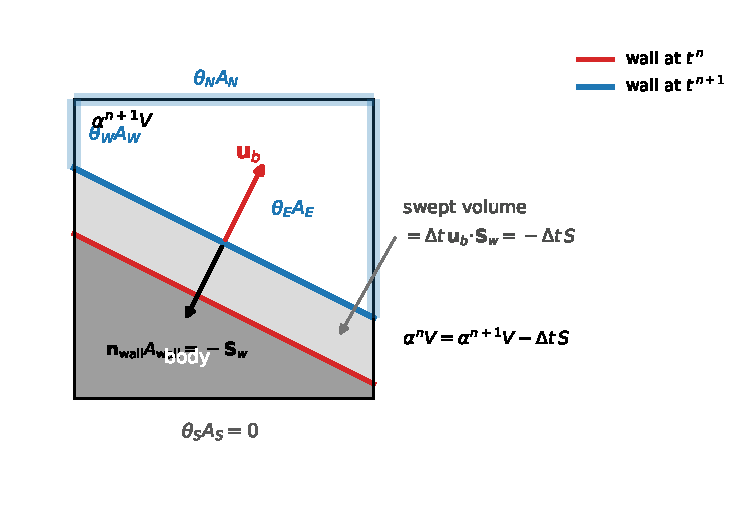
\includegraphics[width=0.58\textwidth]{f1_swept.pdf}
\caption{A cut cell over one step. The faces are fixed in space; only their wet fractions
change. The shaded band is the volume the wall sweeps, $\dt\,\ub\cdot\Sw=\dt S_P$, the only
quantity the motion contributes to the discretisation.}
\label{fig:swept}
\end{figure}

\subsection{Step restriction}

The row sum of unsteady plus convective operator is exactly $\alpha^nV_P/\dt$, which changes
sign when the swept volume exceeds the fluid the cell holds:
\begin{equation}
\dt\,|\ub|\lesssim\frac{\alpha_PV_P}{\Aw}=2\dw .
\end{equation}
This is a condition on the smallest wet cell, hence set by $\alpha_{\min}$ rather than by the
mesh spacing. It is not fatal when violated in a few cells --- the diagonal there is still
dominated by the viscous and wall terms, which grow like $1/\alpha_P$ --- and the solver reports
$\min_P\alpha^n_P$ and the number of violating cells at every step.

\subsection{Rigid body kinematics}

A body is defined at rest and moved by a rigid motion: translation $\bm d(t)$ with velocity
$\bm U(t)=\dot{\bm d}$, optionally a rotation with constant angular velocity $\bm\omega$
about its centre. The velocity must be the exact derivative of the displacement: the first
supplies the wall condition, the second the mass source, and if they disagree the two halves of
the boundary condition pull against each other. Level-set queries are evaluated by transforming
the points into the body frame (inverse translation and rotation), and, in periodic
directions, by taking the minimum image of the point about the current centre, so that a body
may cross a periodic boundary. The same transform gives $\ub(\bm x)=\bm U+\bm\omega\times
(\bm x-\bm c(t))$ at the cell centres. The kinematics may also be set from outside at every
step, which is the hook for a body driven by its own equation of motion.

\section{Passive scalar transport}
\label{sec:scalar}

Integrating \eqref{eq:scalar} over the fluid part of a cell with the same arguments as above
gives
\begin{equation}
\begin{aligned}
\frac{(\alpha^{n+1}_PT^{n+1}_P-\alpha^n_PT^n_P)V_P}{\dt}
+\sum_f\phi_f\bar T_f
-\sum_f\theta_fD_f\delta_f|\Sf|(T_N-T_P)\qquad&\\
+\;D\,\frac{\Aw}{\dw}\,(T_P-T_w)\,[\text{fixed value}]
&=q_P\,\alpha_PV_P ,
\end{aligned}
\label{eq:scalard}
\end{equation}
with $\alpha^n$ the swept fraction \eqref{eq:candB} for a moving body. The wall segment is
seen either as a fixed-value surface --- the analogue of no slip, one diagonal term with the
Dirichlet wall coefficient of Section~\ref{sec:geom} and the source $D\Aw T_w/\dw$ --- or as
a zero-flux surface, the analogue of free slip, which needs no term at all because the wall
segment simply carries no flux. The two masks, for velocity and scalar, are independent. Solid
cells are blanked to $T_w$ so that a cell released by a moving body starts from a defined
value. No mass-source term appears: Reynolds transport gives exactly \eqref{eq:scalard} because
the relative flux through the wall is zero, and a uniform $T$ is preserved for the same reason
as in Proposition~\ref{prop:freestream}. The source $q$ multiplies $\alpha_P$, so it never
injects into the solid.

Cells containing the wall are fluid cells: the scalar is transported into their fluid part
through the wet fraction of their faces and never across the wall segment. The budget
\begin{equation}
\begin{aligned}
&\underbrace{\sum_P\alpha_PV_PT_P}_{\text{content}}
-\underbrace{\sum_n\dt\sum_Pq_P\alpha_PV_P}_{\text{injected}}
+\underbrace{\sum_n\dt\sum_PD\frac{\Aw}{\dw}(T_P-T_w)}_{\text{through walls}}\\
&\qquad+\underbrace{\sum_n\sum_P(\alpha^{\rm prev}_P-\alpha^n_P)V_PT^n_P}_{\text{swept defect}}
=\text{round-off}
\end{aligned}
\label{eq:budget}
\end{equation}
is evaluated at every step. The last term exists only for moving bodies: $\alpha^n$ is
integrated from the wall flux and is first-order consistent with the geometric fraction
$\alpha^{\rm prev}$ of the previous step, and a cell absorbed into the body hands over no
content. It is the price of the exact geometric conservation law of
Section~\ref{sec:primary}, and it is small (Section~\ref{sec:verifscalar}).

\section{Implementation in OpenFOAM}
\label{sec:impl}

\subsection{Explicit operators on an unmodified mesh}

The mesh is left untouched; $\theta_f$ and $\alpha_P$ enter the standard operators
explicitly. The momentum equation of the transient solver reads
\begin{lstlisting}
fvm::ddt(ibm.alpha(), U)                      // alpha V/dt; alpha.oldTime() = alpha^n
+ fvm::div(phi, U)                            // phi = theta (U_f . Sf) = ibm.flux(U)
- fvm::laplacian(ibm.thetaInterpolate(nu), U) // theta-weighted, no wall term
+ fvm::Sp(nu*ibm.noSlipCoeff(), U)            // wall traction, no-slip bodies
+ fvm::Sp(nu*ibm.blankCoeff(), U)             // blanking of solid cells
== fvOptions(U) - ibm.grad(p)                 // sum_f theta_f (p_f - p_P) Sf / V
\end{lstlisting}
and, for moving bodies, \code{UEqn -= ibm.movingWallSource(nu)} adds
$\nu(\text{noSlipCoeff}+\text{blankCoeff})\ub$. The pressure equation is
\begin{lstlisting}
fvm::laplacian(ibm.thetaInterpolate(rAtU), p) == fvc::div(phiHbyA)  // phiHbyA = ibm.flux(HbyA)
pEqn -= ibm.massSource();          // moving bodies only: div(phi) = -S
ibm.constrainPressure(pEqn);       // regular rows for the solid cells
\end{lstlisting}
and \code{pEqn.flux()} is then automatically $\theta$-weighted. Everything else is untouched
\code{simpleFoam} and \code{pimpleFoam}: the boundary constraints on $\bm H/a_P$ and $p$,
the pressure reference, pressure relaxation, fvOptions, residual control and the PIMPLE loops.

This choice keeps the full cell volume $V_P$ in \code{fvMatrix::A()}, so that
$r_A=V_P/a_P$ is exactly the mobility of \eqref{eq:peqn}. Scaling the face area vectors and
cell volumes of the mesh in place would make all operators $\theta$/$\alpha$-aware
implicitly, but would change the SIMPLEC mobility to $\alpha V_P/a_P$, break the interpolation
weights on closed faces and require floors for solid cells; explicit operators are transparent
and term-for-term identical to the formulation above.

The two-level unsteady term of Table~\ref{tab:moving} costs no solver code: the density-weighted
time derivative of OpenFOAM uses the old-time value of the weight in its source, so the swept
fraction $\alpha^n$ of \eqref{eq:candB} is simply stored as the old-time value of $\alpha$
after the geometry update. The transient Rhie--Chow correction (\code{ddtCorr}) is provided in Euler form with
the old flux rescaled to the new wet area.

\subsection{Structure}

\begin{description}\itemsep2pt
\item[\code{ibmBody}] a body: analytical (cylinder, sphere, box, half space), any closed
      \code{searchableSurface} (e.g.\ an STL through \code{triSurfaceMesh}), or a supplied
      fraction field; with its wall conditions and its \code{bodyMotion} (none, translating,
      oscillating, prescribed \code{Function1}, external).
\item[\code{cutCellGeometry}] the fractions and derived fields of Section~\ref{sec:geom}, the
      cut-cell operators (gradient, flux, \code{ddtCorr}), the solid-row regularisation, the
      forces, and \code{update()}, which returns immediately unless a body moves. The
      moving-only fields (body velocity, mass source) are allocated only then, so the static
      path carries no additional cost.
\item[\code{ibmMeanVelocityForce}] constant-flow-rate forcing for periodic domains: the bulk
      velocity is averaged over $\alpha V$, the force acts on the fluid volume only, and the
      controller gain is the SIMPLEC mobility $1/(A-H_1)$, the exact bulk response to a
      uniform force, floored at $\alpha/\dt$; $1/A$ underestimates the response by the
      diffusion number $\nu\dt/h^2$ with implicit viscosity. A zero target is allowed.
\item[\code{ibmScalarTransport}] equation \eqref{eq:scalard}, the per-body wall masks, a
      circular source, and the budget \eqref{eq:budget}.
\item[\code{ibmSimpleFoam}, \code{ibmPimpleFoam}] \code{simpleFoam} and \code{pimpleFoam}
      with the terms above; the moving-body operations sit behind three
      \code{if (ibm.moving())} guards in the transient solver.
\end{description}
The geometry computation is local except for the synchronisation of coupled faces
(\code{syncTools}) and global reductions, so parallel runs need nothing else; a four-rank
run reproduces the serial forces to $2\times10^{-12}$.

\section{Verification}
\label{sec:verif}

All cases use a circular cylinder of radius $R=1$ in a $10\times10$ doubly periodic box
discretised by $81\times81$ cells, $\nu=1$, $\alpha_{\min}=0.02$, central differencing for
convection. The reference is an independent implementation of the same discretisation on a
structured grid (direct sparse solves, exact pinning of the bulk velocity by superposition), so
that the comparison isolates the OpenFOAM implementation from the formulation.

\subsection{Body at rest}

The flow is driven at bulk velocity $0.5$ ($Re_D=1$). Table~\ref{tab:static_verif} compares
geometry, fields and drag. The fractions agree to round-off ($\alpha$ exactly, $\theta$ to
$10^{-11}$, the bisection tolerance). The transient solver run with the reference's
pseudo-time step ($\dt=65h^2/\nu$, Euler, one corrector, SIMPLEC, no \code{ddtCorr}) converges
to the same discrete fixed point (velocity to $10^{-5}$, drag to $2\times10^{-6}$); the steady
solver differs through the relaxation dependence of the Rhie--Chow dissipation. Bodies given as
an STL (a 3600-gon) or as a fraction field give the expected accuracy of their geometry route.
With two bodies of mixed wall conditions the forces sum to the driving force times the fluid
volume to all digits.

\begin{table}[htbp]\centering\footnotesize
\caption{Body at rest, no slip unless stated; reference drag $5.660008$ (no slip), $2.935529$
(free slip), per unit depth and density.}
\label{tab:static_verif}
\setlength{\tabcolsep}{4pt}
\begin{tabular}{@{}lccccc@{}}
\toprule
& steady & transient, ref.\ $\dt$ & STL body & fraction field & free slip\\
\midrule
$\alpha$, cell by cell & exact & exact & exact & exact & exact\\
$\theta$, face by face, max diff. & $7.6\times10^{-11}$ & $7.6\times10^{-11}$ & $6.4\times10^{-6}$ & $0.11$ & $7.6\times10^{-11}$\\
$u$, max diff.\,/\,max $u$ & $2.2\times10^{-4}$ & $9.4\times10^{-6}$ & $2.2\times10^{-4}$ & $3.3\times10^{-3}$ & $1.7\times10^{-5}$\\
drag & $5.660383$ & $5.659997$ & $5.660383$ & $5.651222$ & $2.935496$\\
\bottomrule
\end{tabular}
\end{table}

\begin{figure}[htbp]\centering
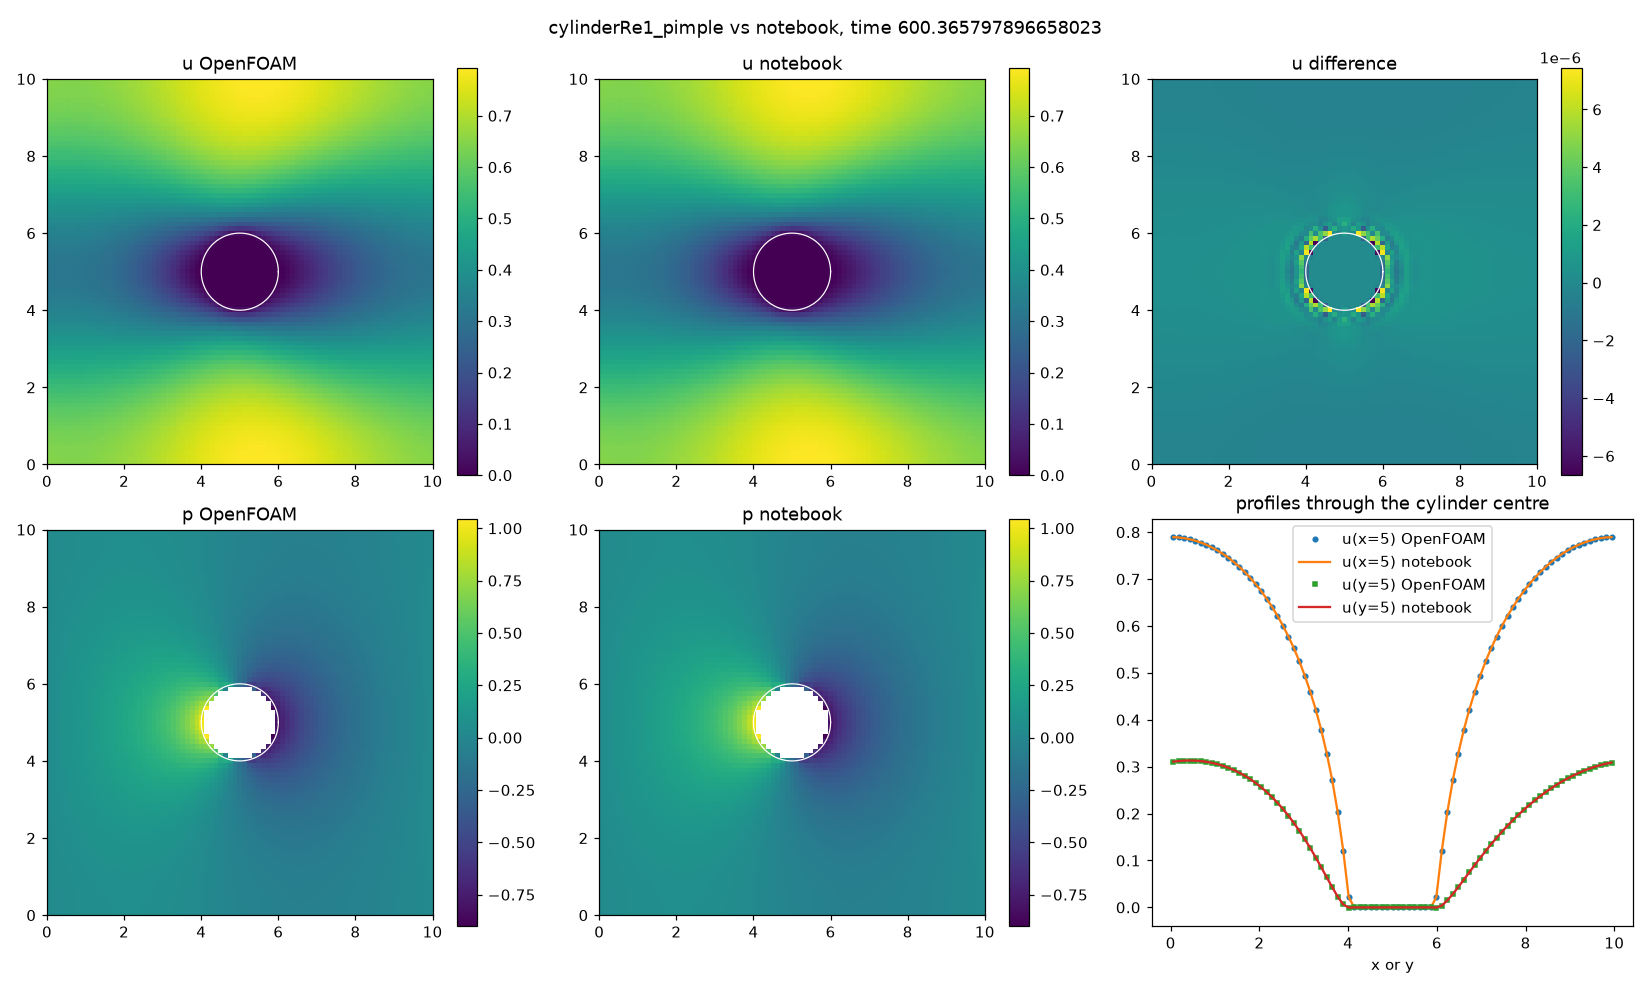
\includegraphics[width=0.98\textwidth]{fig_pimple_vs_notebook.png}
\caption{Body at rest, transient solver with the reference's pseudo-time step: streamwise
velocity (top) and pressure (bottom) against the reference, difference field, and profiles
through the cylinder centre.}
\end{figure}

\subsection{Moving body: free stream, oscillation, Galilean invariance}
\label{sec:galilean}

\emph{Free-stream preservation.} The domain is filled with $\uu=\ub$ and the body translates
at $\ub$ for five steps of $\dt=0.025$ (Proposition~\ref{prop:freestream}). The maximum
departure from $\ub$ over the fluid is $0.0$ in $u$ and below $2\times10^{-15}$ in $v$ for
$u_b=0.37$ and $u_b=2.0$ and for one or three outer iterations; the reference gives
$6\times10^{-16}$ and $4\times10^{-15}$. The test exercises the two-level unsteady term, the
mass source, the moving-wall traction, the blanking and the flux re-interpolation
simultaneously; a sign error in any of them gives an $O(1)$ result.

\emph{Oscillating cylinder.} $x_c=5+\sin(2\pi\cdot0.05\,t)$, $t\in[0,10]$, 400 steps, three
outer iterations, bulk velocity pinned to zero. The force histories agree to
$4.4\times10^{-4}$ after the impulsive first ten steps ($7\times10^{-5}$ of the peak force; the
first step, $F=-60.6$, agrees to $0.2\%$), the driving force to $10^{-6}$, and the final
fields to $2\times10^{-7}$ in velocity (Fig.~\ref{fig:osc}). The mass-source sum and the
continuity error $\max_P|\sum_f\phi_f+S_P|$ are at round-off at every step.

\begin{figure}[htbp]\centering
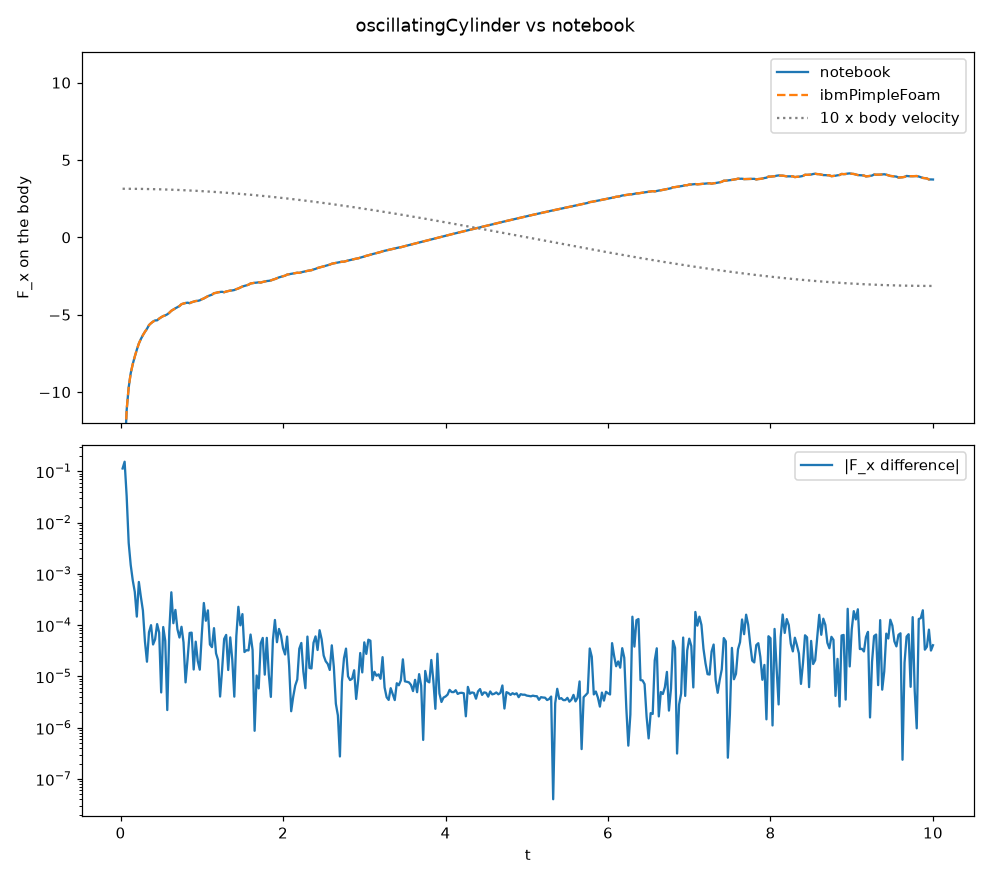
\includegraphics[width=0.8\textwidth]{fig_oscillating_vs_notebook.png}
\caption{Oscillating cylinder: streamwise force on the body against the reference (top) and
their difference (bottom).}
\label{fig:osc}
\end{figure}

\emph{Galilean invariance.} A body translating at $u_b=0.5$ through a fluid of zero bulk
velocity is the Galilean image of the body at rest in a bulk flow of $0.5$, but is computed
through entirely different terms. Over $t\in[0,30]$ the body crosses the periodic seam twice.
The mean force over the last 400 steps is $-5.69099\pm0.0883$, against $-5.69103\pm0.0884$
for the reference and $+5.66038$ for the body at rest: the $0.5\%$ difference between moving
and fixed body is the first-order signature of the $O(\dt)$ swept-volume integration, and the
$\pm1.5\%$ ripple is the body sliding from one cut pattern to the next, the characteristic
signature of a cut-cell method on a non body-fitted mesh. The histories agree to
$1.3\times10^{-3}$ at every step after the impulsive start (Fig.~\ref{fig:gal}).

This test exposed a subtlety of the seam treatment. The reference, as published, copies
$\theta$ across the periodic seam \emph{before} absorbing slivers, so an absorbed cell at
$x=L$ closes its face on that side while the same face stays open for the cell at $x=0$;
while the body front or back crosses the seam its force deviates by up to $2.7\%$ for a few
steps. Synchronising the coupled faces with the minimum \emph{after} absorption
(Section~\ref{sec:geomcomp}) keeps closure exact, the mass-source sum being $10^{-19}$
throughout; applying the same rule to the reference removes the deviations, and the numbers
above are against that reference.

\begin{figure}[htbp]\centering
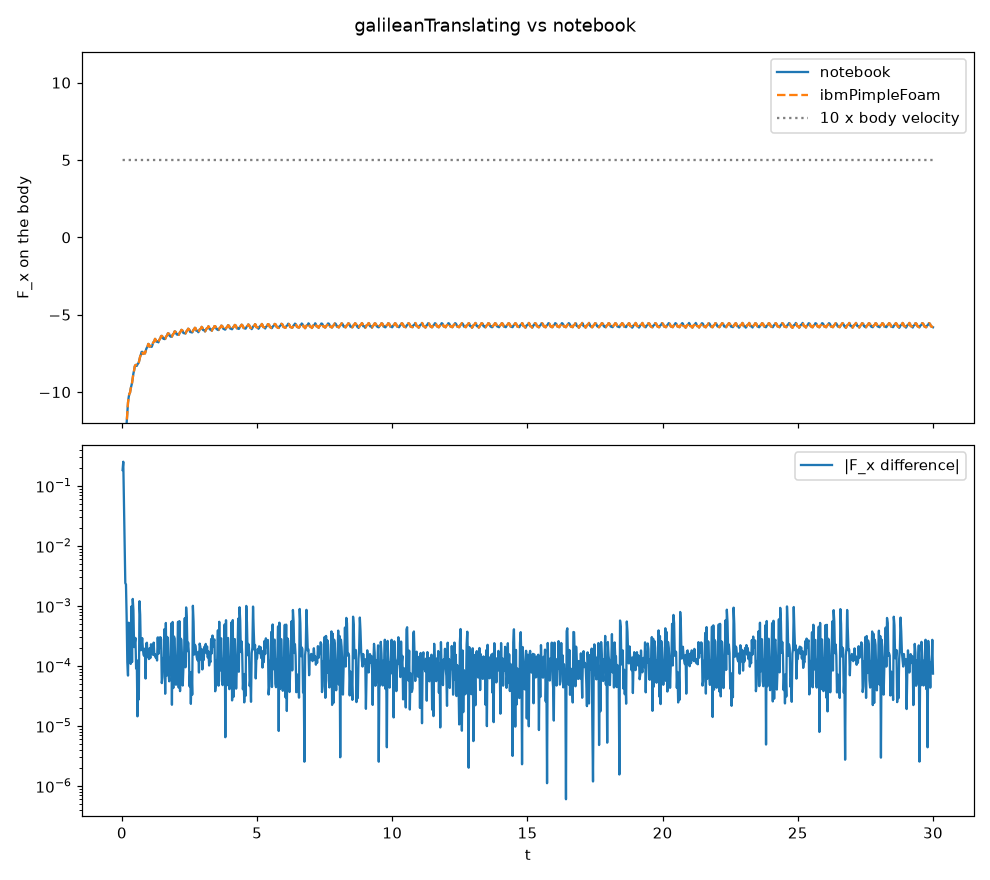
\includegraphics[width=0.8\textwidth]{fig_galilean_vs_notebook.png}
\caption{Translating cylinder crossing the periodic seam twice: force history against the
reference (top) and their difference (bottom).}
\label{fig:gal}
\end{figure}

\subsection{Passive scalar}
\label{sec:verifscalar}

A scalar initially zero is injected at unit rate in a disk of radius $0.5$ centred at
$(5,8.5)$, away from the path of the body, with $D=0.1$, and the budget \eqref{eq:budget} is
followed (Table~\ref{tab:scalar}, Fig.~\ref{fig:scalar}). With zero-flux walls and a body
at rest the content equals the injected amount to $4\times10^{-12}$ after 200 steps and the
solid stays exactly at zero: nothing is lost into the solid. With fixed-value walls the amount
that left through the wall closes the budget to $6\times10^{-11}$, and in the steady solver
the source rate equals the wall flux rate to $10^{-11}$. With a moving body the content differs
from the injected amount by the swept-volume defect only, $3\times10^{-5}$ of the content for
the oscillating cylinder and $8\times10^{-5}$ for the translating one, the solid stays at the
wall value, and the residual budget errors of $10^{-10}$ are accumulated linear-solver
tolerance. The flow is unaffected by the scalar.

\begin{table}[htbp]\centering\footnotesize
\caption{Scalar budget \eqref{eq:budget} at the end of each run.}
\label{tab:scalar}
\setlength{\tabcolsep}{4pt}
\begin{tabular}{@{}lrrrrrr@{}}
\toprule
case & steps & content & injected & through walls & swept defect & budget error\\
\midrule
at rest, zero flux (transient) & 202 & 19.581366 & 19.581366 & 0 & 0 & $-3.9\times10^{-12}$\\
at rest, fixed value & 202 & 11.904949 & 19.581366 & 7.676417 & 0 & $-5.7\times10^{-11}$\\
at rest, fixed value (steady) & 1834 & 16.323010 & rate 0.097847 & rate 0.097847 & -- & $-1.0\times10^{-11}$\\
oscillating, zero flux & 400 & 0.978439 & 0.978472 & 0 & $3.3\times10^{-5}$ & $-8.0\times10^{-11}$\\
oscillating, fixed value & 400 & 0.968143 & 0.978472 & 0.010344 & $-1.5\times10^{-5}$ & $-6.1\times10^{-11}$\\
translating, zero flux & 1200 & 2.935650 & 2.935415 & 0 & $-2.3\times10^{-4}$ & $-7.5\times10^{-10}$\\
\bottomrule
\end{tabular}
\end{table}

\begin{figure}[htbp]\centering
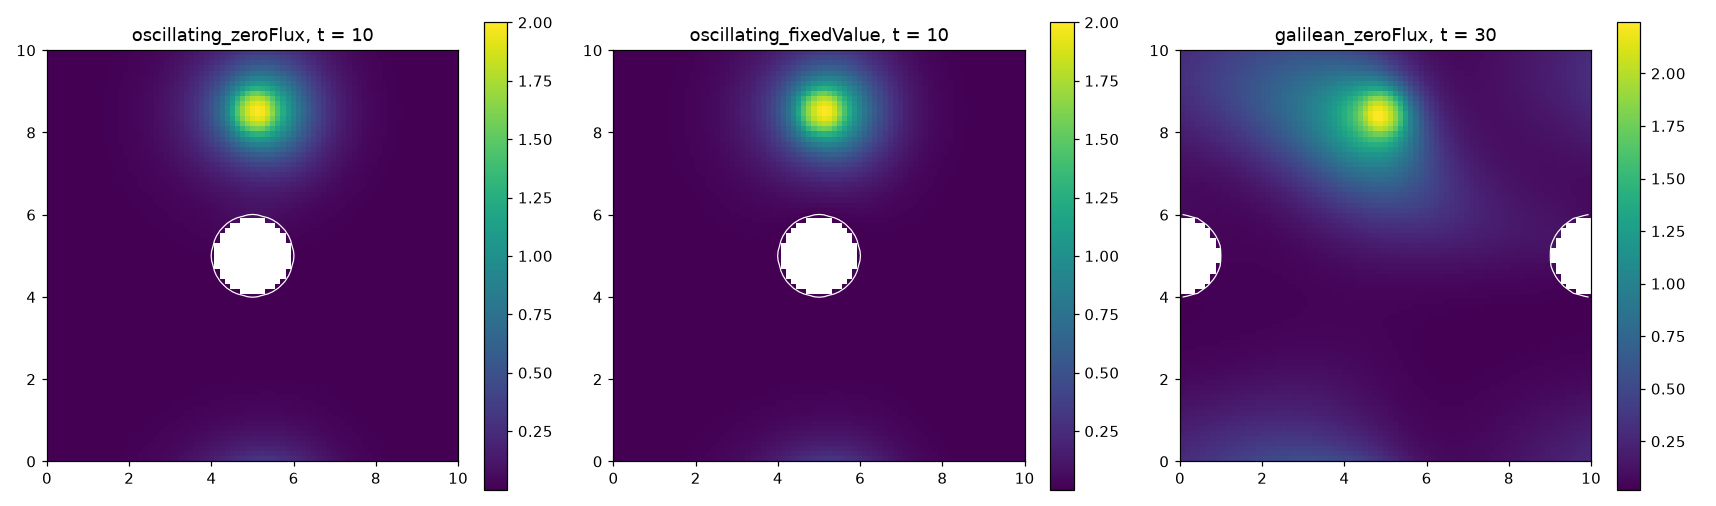
\includegraphics[width=0.98\textwidth]{fig_scalar.png}
\caption{Scalar field for the oscillating cylinder with zero-flux (left) and fixed-value
(centre) wall, and for the translating cylinder with zero-flux wall (right); the body is
blanked.}
\label{fig:scalar}
\end{figure}

\section{Limitations}
\label{sec:limits}

\begin{itemize}\itemsep2pt
\item \emph{Order.} First order in time (implicit Euler, inherited by the swept-volume
      integration) and first order in space for no slip, because of the wall-normal distance
      estimate \eqref{eq:dwall}; free slip is second order. A second-order extension in time
      would need $\alpha$ at three levels and a three-level form of \eqref{eq:candB}.
\item \emph{Slivers.} Absorption below $\alpha_{\min}$ displaces the boundary by
      $O(\alpha_{\min}h)$, and a cell crossing the threshold hands over no momentum or scalar
      content; mass conservation is unaffected. Cell merging is the clean remedy and would
      also relax the step restriction.
\item \emph{Laminar.} Turbulence models are constructed for their effective viscosity only;
      their own transport equations would need the same treatment as the scalar.
\item \emph{Fraction-field bodies.} Reconstructing $\theta$ from the $0.5$ iso-surface of the
      point-interpolated fraction smears the wall over one cell (drag $-0.16\%$ on the
      cylinder); a per-cell iso-value search reproducing each cell's $\alpha$ would bring it to
      $O(h^2)$.
\item \emph{One fluid region.} A single pressure reference; a body splitting the fluid would
      need one per region.
\item \emph{Cost of moving bodies.} The level set is evaluated at all points, face and cell
      centres every step, and $n_s^d$ samples per cut cell; for three-dimensional
      triangulated bodies a smaller $n_s$ or a band around the previous position is advisable.
\end{itemize}

\section{Conclusions}

The method rests on one geometric statement, the closure identity of a cut cell, and on one
choice for moving bodies, the wall flux as the primary quantity. From the first follow
exactness for uniform tangential flow, the absence of spurious pressure forces and
no-penetration itself; from the second follow exact compatibility of the pressure system and
a discrete geometric conservation law that preserves a free stream to machine precision. The
whole boundary treatment adds to the interior scheme two scalar fields, $\theta_f$ and
$\alpha_P$, one diagonal coefficient for a no-slip or fixed-value wall, and one source term
for a moving wall. Implemented in OpenFOAM with explicit operators on an unmodified mesh, it
reproduces an independent reference implementation to the level of the linear-solver
tolerances for a body at rest, oscillating and translating through a periodic boundary, and
transports a passive scalar with a budget that closes to round-off.

\end{document}
